\chapter{Navegación autónoma en seguimiento de rutas 3D}\label{cap.desarrollo}
\hspace{1cm} En este capítulo se describen los pasos seguidos para lograr una solución a los objetivos planteados, utilizando la infraestructura mencionada anteriormente y como se ha implementado.

\hspace{1cm} La solución al problema ha sido un algoritmo de navegación sobre el cual se dará una visión global. A continuación se explicará en detalle el diseño y el funcionamiento de cada uno de los componentes utilizados. Por último, se detallará cómo ha sido el proceso de integración y cual es la estructura del producto final.

%\hspace{1cm} Para explicar todo los pasos primero se dara un vistazo al diseño globalmente para posteriormente explicar cada uno de los modulos indicidualmete y así poder conocer todos ellos en detalle.

\section{Diseño}
\hspace{1cm} El objetivo de este algoritmo es que permitir al drone realizar un comportamiento completamente autónomo desde el despegue, hasta el aterrizaje, ambos controlados, pasando por el seguimiento de una ruta previamente definida. Todo esto basándose únicamente en balizas de apoyo visual. Por lo que estaríamos hablando del vuelo completamente autónomo de un drone mediante visión artificial y control de posición.

\hspace{1cm} En la aplicación final se diferencian dos partes principales: por un lado tenemos el componente encargado de estimar la posición mediante algoritmos de visión por computador y por otro lado tenemos el componente que se encarga del control del drone tomando las decisiones del movimiento según la etapa en la que se encuentre.

\hspace{1cm} En el esquema \ref{fig:Esquema representativo.} se puede ver una explicación de las entradas y salidas de flujos de información. También se pueden observar los ficheros que son imprescindibles en cada modulo para su correcto funcionamiento. Esta imagen nos da una idea del funcionamiento global de la aplicación y se puede observar como toda la comunicación entre procesos se lleva a cabo mediante ICE. A continuación vamos a explicar el comportamiento de cada módulo de una forma breve. 

\begin{figure}[H]
	\begin{center}
		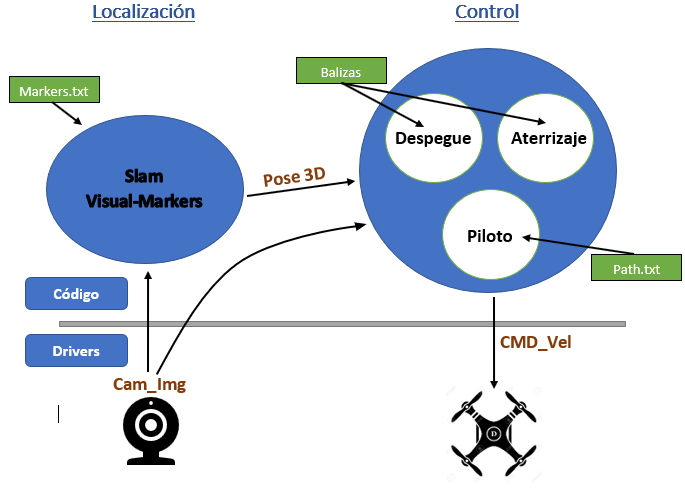
\includegraphics[width=1.1\textwidth]{imag/IMG31.PNG}
				\caption{Esquema representativo de la aplicación.}
		\label{fig:Esquema representativo.}	
	\end{center}
\end{figure}

\hspace{1cm} El módulo Slam VisualMarkers recibe las imágenes que le proporciona el drone y envia los datos en forma de Pose3D(x,y,z,q0,q1,q2,q3) a VisualStates. Este componente comienza analizando la imagen recibida en busca de la presencia de marcadores AprilTags. Si no los encuentra devuelve el número 0 como indicador de ello, en cambio si encuentra alguna envía cuántas ha encontrado y aplica cálculos de geometría proyectiva para estimar la posición de la cámara con respecto a cada una de las balizas. A continuación realiza una fusión espacial, aplicando un filtro basado en pesos y una fusión temporal, mediante un filtro de Kalman. Finalmente, la estimación calculada se envía al componente de navegación mediante una interfaz ICE.

\hspace{1cm} El módulo de Slam VisualMarkers recibe la imagen de la cámara del drone y las posiciones estimadas, envía estos datos a las etapas que lo necesiten y según en la etapa en la que se encuentre genera una serie de órdenes de velocidades que envía al drone vía interfaz ICE para conseguir el objetivo que según la etapa puede ser despegar, aterrizar o seguir una ruta.

\hspace{1cm} A continuación vamos a explicar cada modulo con mayor profundidad, nuestro mayor desarrollo en este TFG fue la creación de un algoritmo de pilotaje que mejorase los anteriores tanto en precisión de seguimiento de rutas como en tiempo de realización de estas rutas, por lo que sera el aparado en el que mas nos centraremos. Sin embargo, al ser un TFG de integración también explicaremos los módulos en los que nos hemos basado y hemos resintonizado para su correcto funcionamiento en el algoritmo final. 

\section{Componente de Autolocazalización} 
\hspace{1cm} Este modulo lo desarrollo originalmente Alberto López Cerón, luego fue refactorizado por Samuel Martín para integrar una capa de comunicaciones mediante interfaces ICE, también añadió métodos para la conversión entre cuaterniones y ángulos de Euler, debido a que la aplicación original utilizaba los ángulos de Euler y la interfaz Pose3D, cuaterniones, posteriormente Manuel Zafra la actualizo para jderobot e hizo los primeros pasos de navegación de drones utilizando esta autolocalización. Por último Felipe Pérez ha cambiado los ficheros de configuración para que sea una herramienta que funcione utilizando únicamente librerías que vienen en JdeRobot por si sola sin depender de QtCreator y su compilador \textit{qmake}, también esta creando la nueva infraestructura en ROS para que se pueda utilizar tanto en ICE como en esta, con la ventaja de que en ROS tendrá nuevos marcadores como el numero de balizas detectadas para poder hacer estudios de precision y marcas temporales para saber cuando entran las balizas en la aplicación y así caracterizar mejor el error de posición. 

\hspace{1cm} En cuanto a la herramienta Slam-VisualMarkers  está formada por un módulo principal \textit{Main-Window} que interconecta el resto de módulos e implementa una interfaz gráfica de usuario. El método \textit{ProcessImage} contenido en \textit{CameraManager} se ocupa de procesar la imagen en 2D capturada por la cámara y buscar en ésta la presencia de marcadores además de estimar la posición 3D con respecto a éstos. Es imprescindible el fichero de Markers.txt que contiene toda la información necesaria de cada marcador: id, tamaño y posición. Para localizar los marcadores en la imagen se hace uso del método de detección ofrecido por la biblioteca AprilTags. Este método se aplica a una versión en escala de grises de la imagen obtenida y tiene como salida un array en el que figuran todos los marcadores encontrados. Una vez el array de marcadores detectados es generado, se aplican una serie de operaciones geométricas. Estas operaciones devuelve la posición relativa de una cámara dado un sistema de referencia compuesto por la correspondencia entre los puntos 2D de la imagen y los correspondientes puntos 3D del mundo De esta forma se obtienen los vectores de translación y rotación del marcador con respecto a la cámara. Finalmente, la matriz que contiene la posición de la cámara con respecto al mundo se obtiene multiplicando la matriz calculada, posición del marcador con respecto a la cámara, y la matriz de posición del mundo con respecto al marcador. 

\begin{figure}[H]
	\begin{center}
		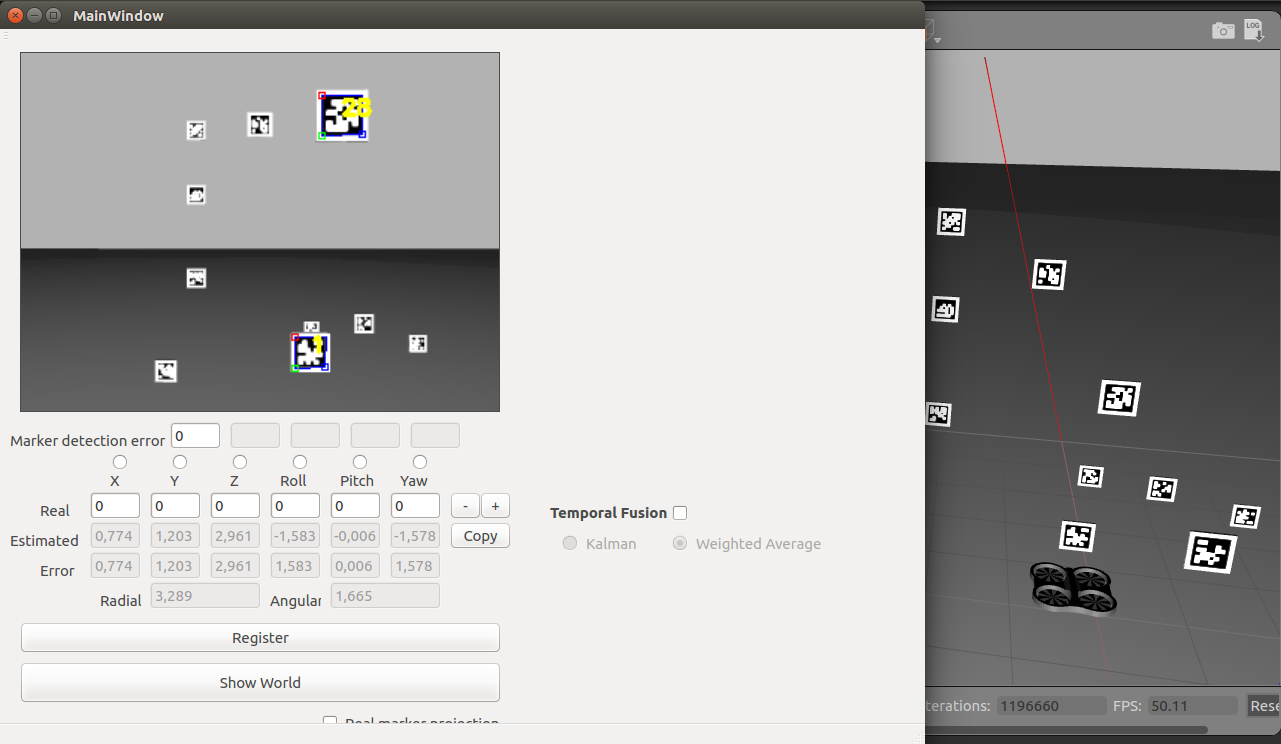
\includegraphics[width=0.85\textwidth]{imag/IMG35.png}
				\caption{Entorno de la aplicación Slam VisualMarkers}
		\label{fig:Ejemplo Slam VisualMarkers.}	
	\end{center}
\end{figure}

\hspace{1cm} Las posiciones estimadas para cada marcador son almacenadas en un array al que es aplicada una fusión espacial mediante un filtro por pesos. Este filtro asigna diferentes pesos a cada estimación basándose en la distancia a la cámara, de forma que los marcadores más cercanos son asignados con un peso mayor. En cuanto a los ángulos de rotación hay una operación especial, ya que no pueden ser sumados de la misma forma que las coordenadas lineales. Por último después de aplicar la fusión espacial, la aplicación original daba opción a aplicar una fusión temporal.  Esta fusión puede llevarse a cabo mediante un filtro por pesos como en el caso de la fusión espacial, o mediante la aplicación de un Filtro de Kalman \cite{FiltroKalman}.

\section{Componente de Control basado en estados}
\hspace{1cm} Todo el algoritmo de la aplicación se ha basado en un componente de control basado en estados, este componente se ha realizado con la herramienta de Visual States, la cual nos ha servido tanto para la creación del código como para la integración del sistema en un solo programa. 

\hspace{1cm} Visual Sates tiene la capacidad de crear estados, donde dentro se encuentra el código que se ejecuta, los cuales recorre mediante transiciones que pueden ser temporales o condicionales. Esto te permite centrarte en la escritura del algoritmo y de la conexión entre estados se encarga la aplicación. Además tiene otros módulos como las constantes y las funciones que una vez creadas se pueden utilizar en todos los estados y transiciones pudiendo así conectar y llevar un seguimiento de lo que ocurre en cada estado. Por último tenemos el apartado de las librerías, en el cual se introducen aquellas de las que depende tu programa, y el apartado de configuración, donde irán los diferentes enlaces a los interfaces de comunicación que hayamos utilizado. 

%\hspace{1cm} Es la parte en la que mas nos hemos centrado y que mas hemos conseguido desarrollar dentro del algoritmo, ya que para nosotros es la parte mas importante. Se podría decir que se trata de un piloto el cual realiza las tareas de pilotaje del drone. Hemos dividido el pilo según los datos que recibe de la interface de VisualStates.

\begin{figure}[H]
	\begin{center}
		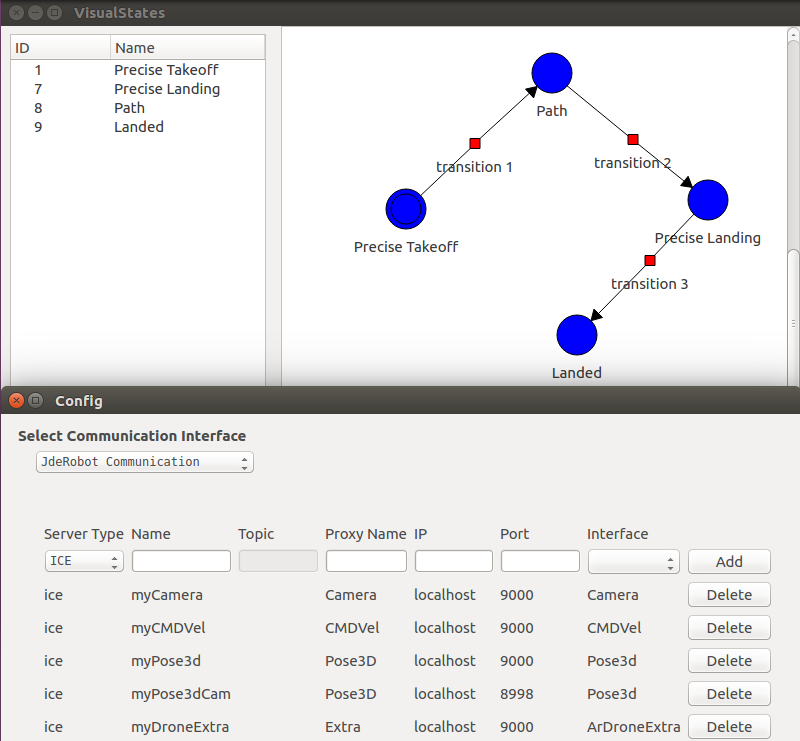
\includegraphics[width=0.8\textwidth]{imag/IMG32.png}
				\caption{Esquema de los componentes de Visual States.}
		\label{fig:Esquema VisualStates.}	
	\end{center}
\end{figure}

\section{Estados de despegue y aterrizaje}
\hspace{1cm} Para este componente hemos utilizado el trabajo que realizó Jorge Vela en su TFG \cite{JorgeVela} refactorizandolo y acoplándolo dentro de nuestro módulo de pilotaje en Visual States. El diseño de este algoritmo es un proceso basado en adquisición-procesado-envío de ordenes.  La adquisición de los datos se realizan mediante los sensores del drone. Estos datos sensoriales serán recogidos para su procesamiento y tras esto se enviarán las instrucciones al drone para que las ejecute. El sensor  utilizado en este estado ha sido la cámara, y a diferencia del estado anterior, los movimientos del drone dependerán de lo que esta capte en cada momento.

\hspace{1cm} El lugar de aterrizaje del drone es una baliza previamente definida \ref{fig:Baliza.}. Esta baliza es un cuadrado que en su interior tiene cuatro cuadrantes, dos verdes, y dos azules. Esta baliza se diseñó así para que sea difícil confundirla con otro objeto, pues de ser una baliza simple se podrían confundir los colores, además lo que busca el software será la cruceta que forman estos cuatro cuadrados y el punto central de ésta.

\begin{figure}[H]
	\begin{center}
		
\includegraphics[width=0.4\textwidth]{imag/IMG33.png}
				\caption{Baliza utilizada en Gazebo.}
		\label{fig:Baliza.}	
	\end{center}
\end{figure}

\hspace{1cm} En cuanto al \textbf{despegue} se sitúa el drone sobre una baliza sobre la cual tiene que estabilizarse. De esta forma, al despegar detecta esta y trata de centrarse, evitando así que se desvíe por factores externos y quedándose en la situación correcta y pasando al siguiente módulo que seria el del piloto. 

\hspace{1cm} Una vez el cuadricóptero termina la ruta establecida, este procede a la siguiente etapa que es el \textbf{aterrizaje}, el cual se divide en dos partes, primero la búsqueda de la baliza de aterrizaje y luego el centrado de la baliza y la aproximación a esta. 

\hspace{1cm} En cuanto a la búsqueda, sigue una navegación en espiral de forma que irá rastreando la zona ampliando su giro de forma continua, hasta que
detecte una baliza. Si no se detecta una baliza, continuará el algoritmo de búsqueda en el punto donde se había quedado, aumentando con la amplitud de las espirales a la que se había llegado. Cuando se detecte, dejara el movimiento en espiral y haciendo que coincida el centro de la baliza con el centro de la imagen de la cámara.  Para realizar el movimiento de centrarse en la baliza se ha utilizado un control PD (proporcional y derivativo).  

\hspace{1cm} por ultimo una vez coincide la cruceta de la baliza con el centro de la imagen, comienza a descender de forma constante a la vez que va centrando imagen por si el drone se desvía por algún factor externo. Cuando el área que detecta la baliza es prácticamente el área de la baliza, en ese momento el drone desciende  hasta  posarse en el suelo, entonces para los motores y el estado cambia a al estado final de \textit{"Landed"}.

\begin{figure}[H]
	\begin{center}
		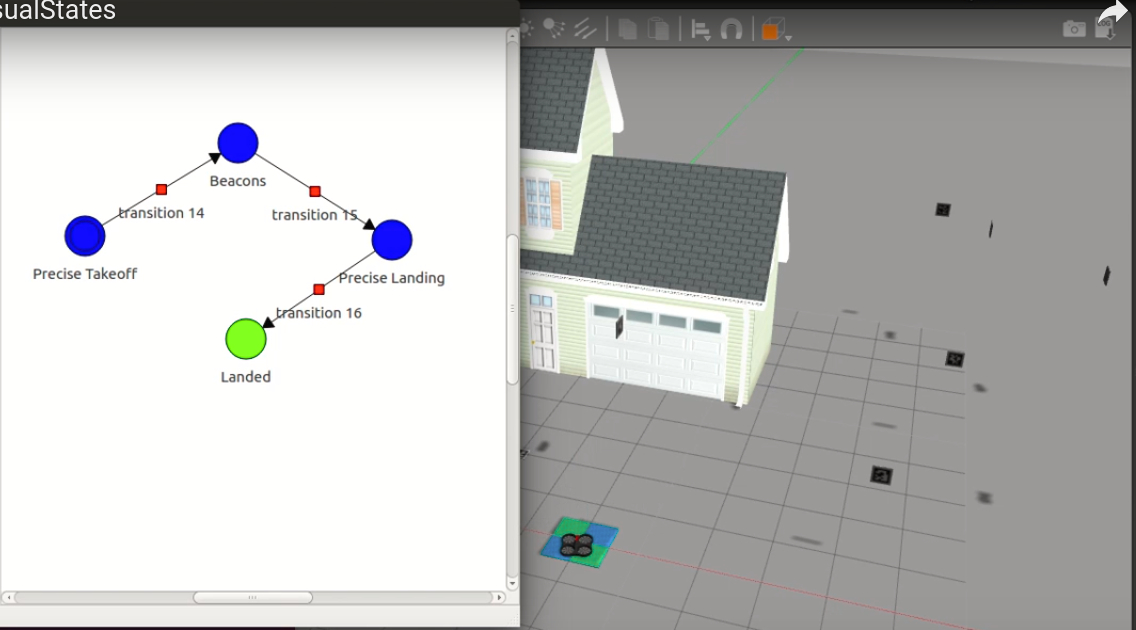
\includegraphics[width=0.9\textwidth]{imag/IMG34.png}
				\caption{Ejemplo de los estados en Visual States}
		\label{fig:Ejemplo Visual States.}	
	\end{center}
\end{figure}

\section{Estado de seguimiento de ruta}
\hspace{1cm} Como se puede observar en la imagen \ref{fig:Esquema VisualStates.} el algoritmo de este componente estaría en el estado de Path, el cual se encarga de seguir una trayectoria. Hemos desarrollado dos algoritmos diferentes según el tipo de trayectoria que se le introduzca, si es una trayectoria de puntos separados en la cual el drone solo tiene que alcanzar esos puntos se trataría del \textbf{Piloto por puntos de paso} si en cambio la trayectoria es una ruta de puntos prácticamente continuos y en la cual queremos que el drone mire hacia el siguiente punto al que se dirige entonces se trataría del \textbf{Piloto por trayectoria}. Ambos algoritmos se basan en la posición tridimensional del drone para ello hemos utilizado los tipos de datos de JdeRobot \textit{Pose3D} los cuales nos devuelven tanto la posición del drone como su orientación en el espacio mediante los cuaterniones o los Ángulos de Euler según lo que necesitemos. Estos datos serán proporcionados por la estimación de posición de Slam VisualMarkers. Y nuestro algoritmo devolvera una serie de velocidades que irá enviando al cuadricóptero mediante la función \textit{CMDVel()}.

\hspace{1cm} Por su sencillez de pilotaje vamos a explicar primero el \textbf{Piloto por puntos de paso}. Este control de pilotaje se centra en el movimiento direccional únicamente, es decir, para que el drone alcance el punto al que debe llegar no variara prácticamente ninguno de sus ángulos de Euler, tan solo se moverá sobre los ejes x,y,z.

\hspace{1cm} Como el movimiento sera únicamente direccional en coordenadas cartesianas tan solo hay que calcular el vector que apunta desde la posición del cuadricóptero hasta el siguiente punto de ruta que se desea alcanzar: 

\[Pose3D = (P_{x}, P_{y}, P_{z})\hspace{1cm};\hspace{1cm}Beacon = (B_{x}, B_{y}, B_{z})\]
\[\overrightarrow{V}_{x} = P_{x} - B_{x}\hspace{0.5cm};\hspace{0.5cm}\overrightarrow{V}_{y} = P_{y} - B_{y}\hspace{0.5cm};\hspace{0.5cm}\overrightarrow{V}_{z} = P_{z} - B_{z}\]

\hspace{1cm} Una vez calculado este vector entre las posiciones lo multiplicaremos por un coeficiente regulador que reducirá los valores hasta que estos se encuentren dentro del rango de velocidades del drone y una vez alcanzado este rango se pasaran los valores por una función que compruebe que las velocidades máximas no exceden las permisibles por Slam VisuaMarkers para la detección y análisis de balizas: 

\begin{lstlisting}[backgroundcolor=\color{gray!15}]
    if math.fabs(xVel) > MaxVx :
        xVel = MaxVx * np.sign(xVel)
    if math.fabs(yVel) > MaxVy :
        yVel = MaxVx * np.sign(yVel)
    if math.fabs(zVel) > MaxVz :
        zVel = MaxVx * np.sign(zVel)        
\end{lstlisting}

\hspace{1cm} Con este método de control de navegación por posición nos aseguraremos que el drone alcanza el punto que queremos adecuadamente y a medida que se va acercando a el, para que la aproximación sea exacta, al reducirse el vector se reducirá la velocidad alcanzando la baliza con total exactitud. Una vez se alcanza la baliza se busca cual es la siguiente en la lista y se vuelve a realizar el proceso, así hasta alcanzar todas ellas.

\hspace{1cm} En cuanto al \textbf{Piloto por trayectoria} lo primero fue crear las rutas que posteriormente seguiría el drone, como estas debían ser largas con giros y con puntos muy consecutivos se creo en python la función que nos permitiese crear estas según la separación entre puntos de ruta que considerásemos necesaria: 
\begin{lstlisting}[backgroundcolor=\color{gray!15}]
i=0
a=0
if i == 0:
    archivo = open('pos.txt','w')
    archivo.write('  x     y     z    roll   pitch   yaw \n')
    i = i+1
b = time.clock()
pos_sim = self.pose.getPose3d()
    if ((b - a) > time_write):
        archivo.write(str(pos_sim.x)+' ')
        archivo.write(str(pos_sim.y)+' ')
        archivo.write(str(pos_sim.z)+' ')
        archivo.write(str(pos_sim.roll)+' ')
        archivo.write(str(pos_sim.pitch)+' ')
        archivo.write(str(pos_sim.yaw)+' ')
        archivo.write(str(b)+'\n')
        a = b 
\end{lstlisting}

\hspace{1cm} Una vez obtenida la ruta y a diferencia del \textbf{Piloto por puntos de paso} este seguirá los puntos orientándose siempre en la dirección entre la posición y el siguiente punto, para ello tendremos que variar la velocidad angular en torno al eje Z, modificando por tanto el ángulo de yaw del drone y de esta forma conseguir orientarlo de la forma mas rápida hasta el siguiente punto de la ruta. Las primeras versiones del piloto tan solo se iban a tener en cuenta las velocidades lineales correspondientes a los ejes X y Z del drone, descartando la velocidad en Y debido a que modificando yaw no sería necesario el movimiento lateral. Pero con forme se fue investigando  mejorando esta versión se descubrió que permitir al drone realizar pequeñas variaciones en la velocidad lineal del eje Y permitía un aproximación a los puntos mucho mas efectiva y precisa, por lo que se optó por incluir también la variación de la velocidad en el eje Y. Con la ayuda del piloto anterior y teniendo en cuenta las mejoras anteriores se va a explicar el algoritmo final de pilotaje. 

\hspace{1cm} Para el cálculo de las velocidades lineales se seguirán los mismos pasos que en el \textbf{Piloto por puntos de paso} pero variaremos los coeficientes de corrección para que las velocidades lineales sean parejas a la nueva velocidad angular. Esta velocidad angular se calculara mediante las funciones de predicción de posición. 

\hspace{1cm} Para ello el primer paso es calcular la distancia horizontal que recorrerá el drone hasta la siguiente iteración del algoritmo. La distancia se obtiene multiplicando la velocidad horizontal obtenida anteriormente por el tiempo que transcurre entre dos iteraciones: \(d_{\psi} = v_{x} * \Delta_{t}\).

\hspace{1cm} Para predecir la posición del cuadricótpero debemos tener en cuenta el ángulo de giro con respecto al eje Z del drone en ese instante. Ya que en el estándar de Pose3D la orientación se indica en cuaterniones, haremos un conversión para conocer el ángulo de Euler mediante la siguiente ecuación:

\[ \Psi_{z} = arctan^{2}\left( \frac{2*q_{0}*q_{3}+q_{1}*q_{2}}{1-2*(q_{2}^{2}+q_{3}^{2})}\right) \]
 
\hspace{1cm} Una vez obtenido el ángulo $\Psi_{z}$ sacamos la posición que predecimos solo en X e Y ya que la variación en Z no influye en cálculo del ángulo de giro de yaw.

\[ X_{f} = d_{\psi} * cos \Psi_{z} + x_{pose} \] 
\[ Y_{f} = d_{\psi} * sin \Psi_{z} + y_{pose} \]

\hspace{1cm} Ahora calcularemos el error de ángulo, que es la diferencia entre el ángulo actual y el ángulo sobre el eje Z existente entre el drone y el punto de ruta, $\Psi_{e}$ Teniendo el ángulo se calcula una velocidad angular a partir de la distancia horizontal al punto, $d_{H}$, y la velocidad lineal actual, $v_{x}$.
 
\[\Psi_{path} = arctan \left(\frac{V_{y}}{V_{x}}\right)  \hspace{0.5cm};\hspace{0.5cm}\Psi_{e} = \Psi_{path} - \Psi_{z} \]

\[d_{H} = \sqrt{V_{x}^{2} + V_{y}^{2}} \hspace{0.5cm};\hspace{0.5cm} \omega_{e} =  \dfrac{\Psi_{e}}{d_{H}/v_{x}}\]

\hspace{1cm} La velocidad angular dependerá entonces de la velocidad angular calculada y de un factor de corrección que viene dado por la relación entre el error lateral predicho $L_{fe}$ y la velocidad horizontal. Este factor está multiplicado por una constante $K_{g}$, que es la ganancia de corrección del giro.

\[ L_{fe} = cos\Psi_{z}*(Y_{path}-Y_{f}) - sin\Psi_{z}*(X_{path}-X_{f}) \]
\[ \omega_{z} = \omega_{e} + K_{g} * (L_{fe}/v_{x})\]

\hspace{1cm} Por último, una vez obtenida la velocidad angular $\omega_{z}$ ajustaremos la velocidad en el eje Y, $v_{y}$, a partir de esta. Una vez obtenidas las tres velocidades que se van a enviar al drone, las velocidades horizontales $v_{x}$ $v_{y}$, la velocidad vertical $v_{z}$ y velocidad angular $\omega_{z}$ se envían al drone mediante una llamada al método \textit{SendCMDVel(vx,vy,vz,wz)}
de Interfaces, que se ocupa de mandar las órdenes decididas al cuadricóptero.
